\documentclass[12pt,a4paper,openright,twoside]{report}


\usepackage[british]{babel}
\usepackage[utf8]{inputenc}


\usepackage{fancyhdr}
\usepackage{indentfirst}
\usepackage{graphicx}
\usepackage{newlfont}
\usepackage{xcolor}


\usepackage{amssymb}
\usepackage{amsmath}
\usepackage{latexsym}
\usepackage{amsthm}


\oddsidemargin=30pt 
\evensidemargin=20pt
\hyphenation{sil-la-ba-zio-ne pa-ren-te-si}
\pagestyle{fancy}\addtolength{\headwidth}{20pt}
\renewcommand{\chaptermark}[1]{\markboth{\thechapter.\ #1}{}}
\renewcommand{\sectionmark}[1]{\markright{\thesection \ #1}{}}
\rhead[\fancyplain{}{\bfseries\leftmark}]{\fancyplain{}{\bfseries\thepage}}
\cfoot{}
\linespread{1.3}


%%%%%%%%%%%%%%%%%%%%%%%%% DEDICATION %%%%%%%%%%%%%%%%%%%%%%%%%%%%%%%%%%%%%%%

\begin{document}

\begin{titlepage}
\thispagestyle{empty}                   
\topmargin=6.5cm                        
\raggedleft                             
\large                                  
                                       
\em                                     
To my beloved\\
Benedetta                   
\newpage                                

\clearpage{\pagestyle{empty}\cleardoublepage}
\end{titlepage}
\pagenumbering{roman}


            




%%%%%%%%%%%%%%%%%%%%%%% INTRODUCTION %%%%%%%%%%%%%%%%%%%%%%%%%%%%%%

\chapter*{Introduction}   
\addcontentsline{toc}{chapter}{Introduction}
\rhead[\fancyplain{}{\bfseries Introduction}]{\fancyplain{}{\bfseries\thepage}}\lhead[\fancyplain{}{\bfseries\thepage}]{\fancyplain{}{\bfseries Introduction}}




  \textcolor{blue}{
    Issues with the current state of machine learning research. Category theory as a unifying force. See  \cite{shieblerCategoryTheoryMachine2021}
  }





%%%%%%%%%%%%%%%%%%%%%%% ITALIAN TRANSLATION OF THE INTRODUCTION %%%%%%%%%%%%%%%%%%%%%%%%%%%%%%


\chapter*{Introduzione}
\addcontentsline{toc}{chapter}{Introduzione}
\rhead[\fancyplain{}{\bfseries Introduzione}]{\fancyplain{}{\bfseries\thepage}}\lhead[\fancyplain{}{\bfseries\thepage}]{\fancyplain{}{\bfseries Introduzione}}





  Questa \`e l'introduzione.







%\clearpage{\pagestyle{empty}\cleardoublepage}


%%%%%%%%%%%%%%%%%%%%%%%%%%%%% TABLE OF CONTENTS %%%%%%%%%%%%%%%%%%%%%%%%%%%%%%

\tableofcontents
\rhead[\fancyplain{}{\bfseries\leftmark}]{\fancyplain{}{\bfseries\thepage}} \lhead[\fancyplain{}{\bfseries\thepage}]{\fancyplain{}{\bfseries Table of Contents}}
%\clearpage{\pagestyle{empty}\cleardoublepage}

\listoffigures                         
%\clearpage{\pagestyle{empty}\cleardoublepage}


\listoftables                           
%\clearpage{\pagestyle{empty}\cleardoublepage}





%%%%%%%%%%%%%%%%%%%%%%%%%%%% FIRST CHAPTER %%%%%%%%%%%%%%%%%%%%%%%%%%%%%%%%%


\chapter{Categorical Toolkit}
\lhead[\fancyplain{}{\bfseries\thepage}]{\fancyplain{}{\bfseries\rightmark}}
\pagenumbering{arabic}







  This is the first chapter.



  \section{Categories}                 
  This is the first section.

  \begin{figure}[h]
    \begin{center}                         
      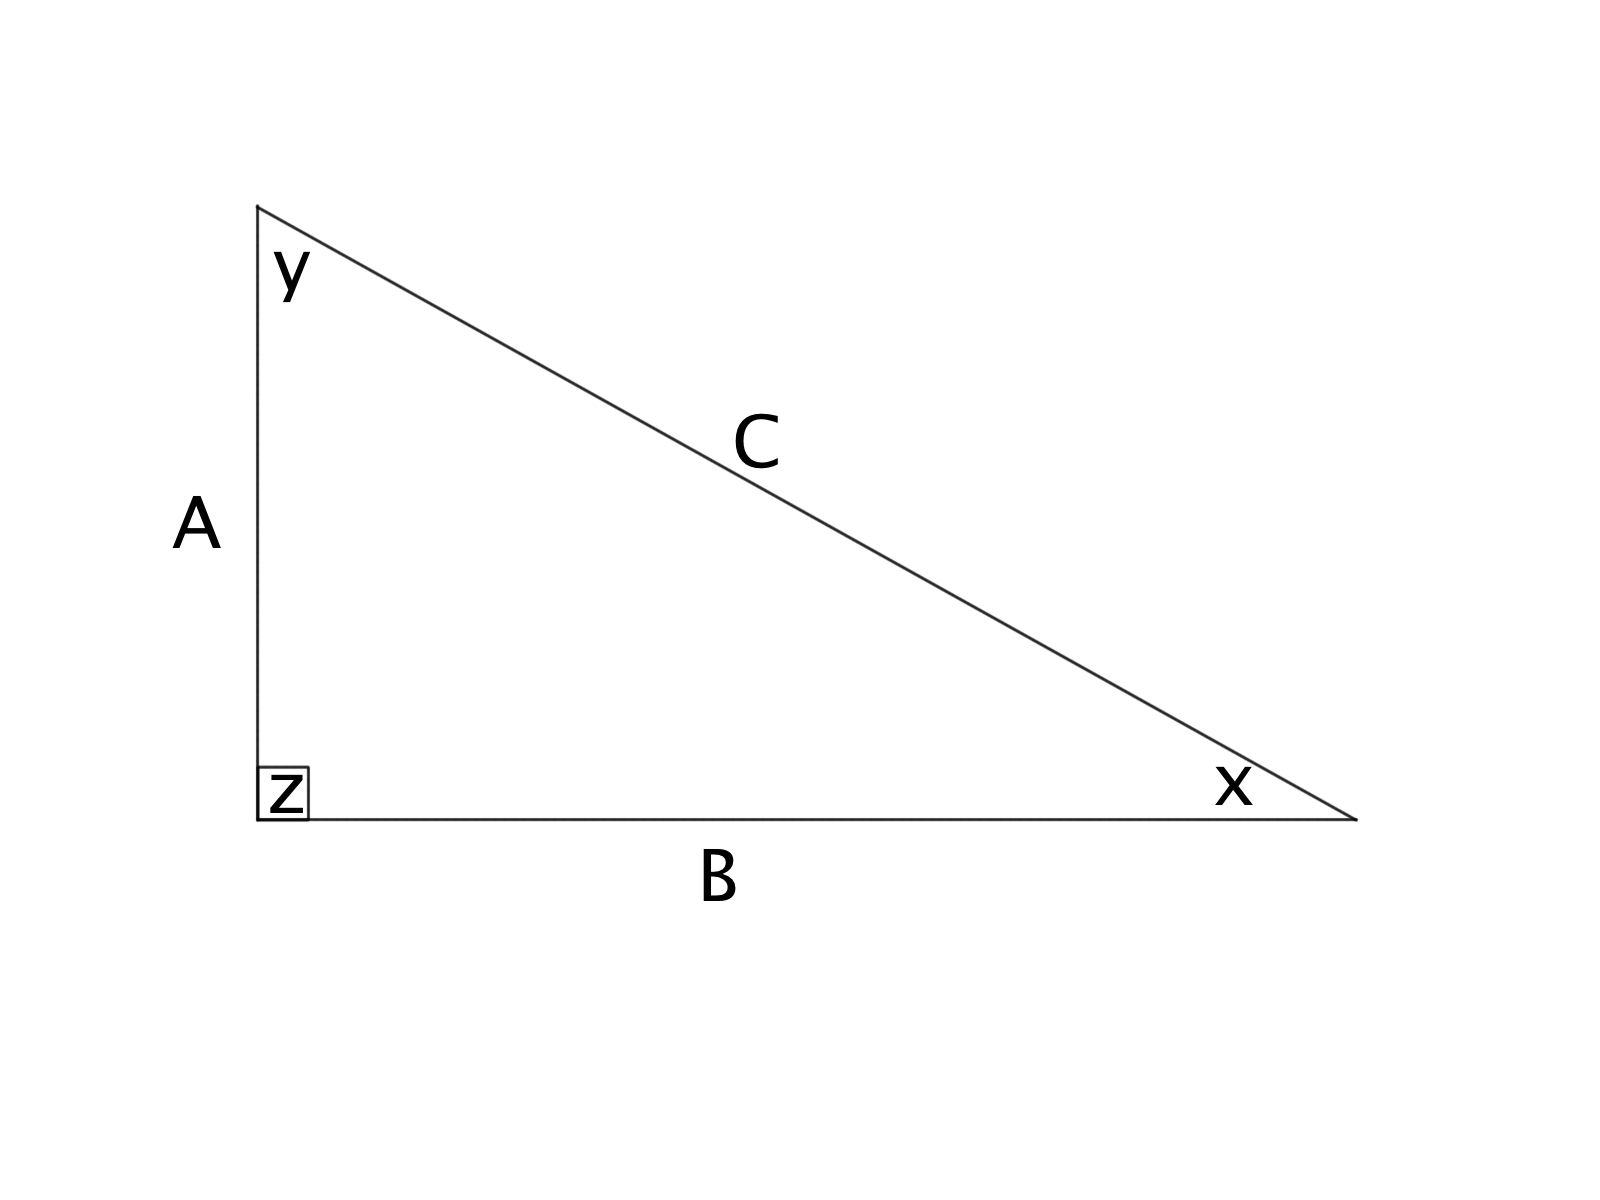
\includegraphics[width=5cm]{figures/triangle.jpg}
      \caption[Placeholder]{Placeholder figure.}\label{fig:first}
    \end{center}
  \end{figure}

  Create the placeholder table \ref{tab:uno}.

  \begin{table}[h]                        
    \begin{center}                          
      \begin{tabular}{r|c|c}                  
        \hline \hline                           
        $(1,1)$ & $(1,2)$ & $(1,3)$\\           
        \hline                                  
        $(2,1)$ & $(2,2)$ & $(2,3)$\\           
        \hline                                  
        $(3,1)$ & $(3,2)$ & $(3,3)$\\
        \hline \hline                           
      \end{tabular}
      \caption[Placeholder Table]{Placeholder table.}\label{tab:uno}
    \end{center}
  \end{table}







%\clearpage{\pagestyle{empty}\cleardoublepage}

%%%%%%%%%%%%%%%%%%%%%%%%%%%%%% CONCLUSIONS %%%%%%%%%%%%%%%%%%%%%%%%%%%%%%%%%%%

\chapter*{Conclusions}
\rhead[\fancyplain{}{\bfseries
Conclusions}]{\fancyplain{}{\bfseries\thepage}}
\lhead[\fancyplain{}{\bfseries\thepage}]{\fancyplain{}{\bfseries Conclusions}}
\addcontentsline{toc}{chapter}{Conclusions} 




This is the conclusion.





%%%%%%%%%%%%%%%%%%%%%%%%%%%%%%%%%%%%% BIBLIOGRAPY %%%%%%%%%%%%%%%%%%%%%%%%%%%%%%

\bibliographystyle{alpha}
\bibliography{references}
\rhead[\fancyplain{}{\bfseries \:Bibliography}]{\fancyplain{}{\bfseries\thepage}} 
\addcontentsline{toc}{chapter}{Bibliography}



% \clearpage{\pagestyle{empty}\cleardoublepage}



%%%%%%%%%%%%%%%%%%%%%%%%%%%%%%%%%%%%%%% ACKNOWLEDGEMENTS %%%%%%%%%%%%%%%%%%%%%%%%%%%

\chapter*{Acknowledgements}

\thispagestyle{empty}

  Placeholder 



\end{document}
